\documentclass[letterpaper, 10pt]{report}
\title{Clemson Cyber Defense Hack Pack}
\author{Clemson ACM}
\date{\today}

\usepackage{makeidx}
\usepackage{multicol}
\usepackage{geometry}
\usepackage{tabularx}
\usepackage{pdfpages}
\geometry{margin=1in}

% Custom command for inline code.
\newcommand{\code}[1]{\texttt{#1}}

% Paragraph spacing should be easy!
\usepackage{parskip}

% Chapter title format: "X. Chaptertitle", not "Chapter X\nChaptertitle".
% Also, make \sections stand out a bit more.
\usepackage{titlesec}
\titleformat{\chapter}[block]{\normalfont\huge\bfseries}{\thechapter.}{1em}{\Huge}
\titleformat{\section}[block]{\normalfont\large\bfseries}{\thesection.}{1em}{\LARGE}

% Adjust spacing around headers to reduce empty space
\titlespacing*{\chapter}{0pt}{-22pt}{-1pt}
\titlespacing*{\section}{0pt}{10pt}{0pt}
\titlespacing*{\subsection}{0pt}{10pt}{0pt}
\titlespacing*{\subsubsection}{0pt}{0pt}{0pt}

% Citations should use superscript. It's nice.
\usepackage[superscript, biblabel]{cite}

% Use the Bera font family (based on Bitstream Vera) for text (bera), captions
% (berasans), and code (beramono).
\usepackage{bera}
\usepackage[scaled]{berasans}
\usepackage[scaled]{beramono}
\usepackage[T1]{fontenc}

% Needed for the inclusion of graphics.
\usepackage{graphicx}

% Allows the use of EPS files, a type of vector graphic.
\usepackage{epstopdf}

% Use the listings package for pretty source code inclusions.
\usepackage{color}
\usepackage{xcolor}
\usepackage{soul}
\usepackage{listings}
\lstset{
  basicstyle=\footnotesize\ttfamily, % Use a truetype, footnote-sized font.
  numbers=left,                      % line numbers go on the left
  numbersep=10pt,                    % how far the line-numbers are from the code
  tabsize=2,                         % sets default tabsize to 2 spaces
  extendedchars=true,                % lets you use non-ASCII characters; for 8-bits encodings only
  breaklines=true,                   % sets automatic line breaking
  keywordstyle=\bfseries,            % Keyword styling
  numberstyle=\ttfamily\color{gray}, % the style that is used for the line-numbers
  stringstyle=\color{gray},          % string literal style
  commentstyle=\itshape\color{gray}, % comment literal style
  title=\lstname,                    % show the filename of files included with \lstinputlisting
  frame=b,                           % show a frame along the bottom
  rulecolor=\color{lightgray},
  language=C++,                      % the default language of the code
  showspaces=false,                  % show spaces as space, not a litle underscore.
  showstringspaces=false             % same as above, in strings.
  showtabs=false,                    % same as above, with tabs.
  xleftmargin=17pt,
  framexleftmargin=17pt,
  framexrightmargin=5pt
}

% Listings caption configuration.
\usepackage{caption}
\DeclareCaptionFont{white}{\color{white}}
\DeclareCaptionFormat{listing}{\colorbox[cmyk]{0.43, 0.35, 0.35,0.01}{\parbox{\textwidth}{\vspace{1.5pt}\hspace{10pt}#1#2#3}}}
\captionsetup[lstlisting]{format=listing,labelfont=white,textfont=white, singlelinecheck=false, margin=0pt, font={bf, sf}}

% Defines a tikz frame for page-broken listing hints.
% Shamelessly stolen from https://tex.stackexchange.com/questions/77996/how-to-show-a-hint-when-lstlisting-is-breaking-page
\usepackage[framemethod=tikz]{./formatting/mdframed}
\mdfdefinestyle{note}
  {
    hidealllines = true ,
    skipabove    = .5\baselineskip ,
    skipbelow    = .5\baselineskip ,
    singleextra  = {} ,
    firstextra   = {
      \node[right,overlay,align=center,font=\continuingfont]
        at (O) {\continuingtext};
    } ,
    secondextra  = {
      \node[above right,overlay,align=left,font=\continuingfont]
        at (O |- P) {\continuedtext};
    } ,
    middleextra  = {
      \node[right,overlay,align=left,font=\continuingfont]
        at (O) {\continuingtext};
      \node[above right,overlay,align=left,font=\continuingfont]
        at (O |- P) {\continuedtext};
    }
  }

% Sets up the hint content and style for page-broken listings.
\newcommand*\continuingfont{\color{gray}\footnotesize\itshape}
\newcommand*\continuingtext{Continues on next page}
\newcommand*\continuedtext{Continued from previous page}

% A wrapper command for automatically wrapping input listings
% with a hintable frame.
\newcommand{\acmlisting}[2][]
{
\mdframed[style=note]
\lstinputlisting[#1]{#2}
\endmdframed
}

% Turn on the powerful indexing features
\makeindex

% Make links, footnotes, etc. clickable, and generate pdf bookmarks.
\usepackage{hyperref}
\hypersetup{
  pdfauthor={Clemson ACM, acm@cs.clemson.edu},
  pdfcreator={Clemson ACM, acm@cs.clemson.edu},
  pdftitle={Clemson ACM Hack Pack},
  pdfsubject={Clemson ACM Hack Pack},
  unicode=true,
  colorlinks=false,
  pdfborder=0 0 0,
  bookmarks=true
}



\begin{document}
\maketitle

#ifdef hackpackpp
\section*{Copyright}
Copyright (C) 2015 CLemson ACM \\
The contents of the .tex files are under a Creative Commons Attribution-ShareAlike 4.0
International License (CC-BY-SA 4.0). 
See https://creativecommons.org/licenses/by-sa/4.0/ for a copy of the license.

The content of all other files is available under the GPLv3 unless otherwise specified. \\
The Hackpack is a concise and extensive cheatsheet/guide designed to be used during cyber security competitions. \\
Copyright (C) 2015  Clemson ACM \\

This program is free software: you can redistribute it and/or modify
it under the terms of the GNU General Public License as published by
the Free Software Foundation, either version 3 of the License, or
(at your option) any later version.

This program is distributed in the hope that it will be useful,
but WITHOUT ANY WARRANTY; without even the implied warranty of
MERCHANTABILITY or FITNESS FOR A PARTICULAR PURPOSE\@.  See the
GNU General Public License for more details. \\

You should have received a copy of the GNU General Public License
along with this program.  If not, see <http://www.gnu.org/licenses/>.

\break
#endif



\begingroup
\let\clearpage\relax
\chapter*{10 Commandments of Cyber Defense}
\begin{multicols}{2}
\begin{enumerate}
    \item Thou shalt NEVER trust the red team
    \item Thou shalt trust but verify everything else
    \item Thou shalt know thy network
    \item Thou shalt patch your S!
    \item Thou shalt make frequent backups
    \item Thou shalt disable unused services
    \item Thou shalt set and use strong passwords
    \item Thou shalt always use a firewall
    \item Thou shalt log everything
    \item Thou shalt get your injects done on time
\end{enumerate}
\end{multicols}
\endgroup


\tableofcontents

\chapter{First 30 Minutes}
\section{Linux Checklist}
This checklist is designed for the first 30 minutes of competition.

For each system:
\begin{itemize}
	\item Change the password for the root account
	\item Check for improper ssh config
	\item Check for improper sshd config
	\item Check the crontab (s) for running tasks
	\item Check with files with wider permissions and setuid
	\item Create a report of running services and processes and disable unnecessary processes
	\item Create a report of open ports
	\item Audit user, groups for invalid entries
	\item Check mount/nfs if it is running
	\item Install Updates
	\item Run a full system backup
	\item Check/Configure sudo and /etc/sudoers.d
	\item Harden the service for your machine
	\item Install/Configure a firewall
	\item Write an audit report containing changes made
	\item Configure ansible
\end{itemize}

For all systems:
\begin{itemize}
	\item Scan the subnet for running servers
	\item Configure a provisioner such as Salt/Ansible master
\end{itemize}


\chapter{Essential Tools}

\section{Shells}
The shell is the primary means of running tasks on Linux and Unix systems.
Bash is the most common shell.

\subsection{Bash}\index{shell!bash}

\subsubsection{Background}
Often you will want to be able to run processes in the background during the contest.
There are a few ways to do this:

\begin{itemize}
	\item Job Control - this is the legacy job control system.
	\item tmux/screen - if they are installed, these are more full featured tools
\end{itemize}

\acmlisting[caption=Job Control,label=Job Control]{./tools/shell/bash/scripts/job_control.sh}

\subsubsection{Scripting}

\acmlisting[caption=Scripting,label=Scripting]{./tools/shell/bash/scripts/scripting.sh}


\section{Provisioners}

Provisioners are tools that allow for specifying configurations that should be applied to a collection of machines.
They can save alot of time from manipulating configurations for several different machines.
Many are available in the package repositories for various Linux distributions.
Some are even available in Windows and BSD.
Some common provisioners are Ansible and Puppet.

\subsection{Ansible}\index{provisioner!ansible}
Ansible is a lightweight agent-less provisioner that uses Python 2.X and OpenSSH as a backend.
It is configured using Playbooks which are files written in a dialect of YAML.

\subsubsection{Setting it up}

\paragraph{Managed Windows Machines}
Ansible can also manage Windows machines running PowerShell 3.0 or later.
For windows machines, you will also need to create an encrypted host\_vars or group\_vars file on the control machine that contains the following information:

\acmlisting[caption=Ansible Windows, label=Ansible Windows]{./tools/provisioners/ansible/scripts/ansible-vault.sh}

It is also required to run the ConfigureRemotingForAnsible.ps1 from the Ansible source code script on the Windows machines that will be managed.
\paragraph{Managed Linux Machines}
Ansible is agent less, this means that only one machine must have Ansible installed on it.
For Linux or BSD managed machines, all you have to have is OpenSSH and Python 2.X.
For some Linux distributions where Python 3.X is the default or python is installed in an non-standard location, you may need to set ansible\_python\_interpetor $=$ /usr/bin/python2.
For best performance, sftp must be enabled in /etc/ssh/sshd\_config as a subsystem with the path to the sftp-server binary

\paragraph{Control Machine}
The control machine must have a few more pieces of software.
On most distributions, it can be installed from package repositories.
It can also be installed from source:

\acmlisting[caption=Ansible Install, label=Ansible Install]{./tools/provisioners/ansible/scripts/ansible-install.sh}

\subsubsection{Inventory Management}
The collections of machines that are managed via Ansible are called the inventory.  Here is an example inventory file:

\acmlisting[caption=Ansible Hosts, label=Ansible Hosts]{./tools/provisioners/ansible/scripts/ansible-hosts.example}


In this example we demonstrate, 
\begin{itemize}
	\item A set of hosts specified by a range of ip addresses
	\item A set of hosts specified by domain name
	\item A host using a different user and default port.
	\item Targeting the localhost
	\item Four groups of hosts called web, webservers, databases, and local
	\item A group of groups called web that contains all the hosts in webservers and databases.
\end{itemize}
NOTE, group variables and host variables can also be specified in the hosts file as shown with the ansible\_connection example, but this format is discouraged because it does not follow a separation of concerns.

\subsubsection{Sample Playbooks}

Repositories containing Ansible playbooks  are generally arranged out as follows:

\begin{itemize}
\item site.yml --- the primary playbook.
\item hosts --- the primary host inventory.
\item group\_vars/ --- directory containing encrypted group variables.
\item host\_vars/ --- directory containing encrypted host variables.
\item roles/ --- directory containing roles that will be applied.
\end{itemize}

Here is an example playbook:
\acmlisting[caption=Ansible Playbook, label=Ansible Playbook, ]{tools/provisioners/ansible/scripts/ansible-playbook.yml}

These playbooks can also be split into separate sections in what are called roles.
Here is how a sample role, in this case a webserver are stored:
\begin{itemize}
\item roles/webserver --- directory where the webserver role is stored.
\item roles/webserver/files --- files that would be referenced via copy commands in the role.
\item roles/webserver/tempates --- templates that would be referenced via template commands in the role.
\item roles/webserver/tasks --- where tasks for the webserver role are stored.
\item roles/webserver/handlers --- where handlers that kickoff post processing tasks for the webserver role are stored.
\item roles/webserver/vars --- where role specific variables for the webserver role are stored.
\item roles/webserver/defaults --- where role specific default values variables for the webserver role are stored.
\item roles/webserver/meta --- where role specific meta data for the webserver role are stored such as dependencies could be listed.
\end{itemize}

\paragraph{Ansible Vault}
Ansible has a means of creating AES encrypted files for use of storing configuration.
To create a file use \lstinline|ansible-vault create <filename>|
To edit a file use \lstinline|ansible-vault edit <filename>| which will open the file un-encrypted in the user's EDITOR and re-encrypt it after editing.
It can be used for file containing variables and files that are part of roles.

\paragraph{Extending Ansible}
Somethings Ansible is just not good at, string parsing for instance.
You can write modules in Python that do this heavy lifting.
Here is a sample module that checks for the sshd version, and sets a variable with the output

\acmlisting{./tools/provisioners/ansible/scripts/ansible-facts-module.py}

\paragraph{Documentation}
For each of the ansible modules, there is documentation that is installed.
It can be viewed using the \lstinline|ansible-doc| command.
Use \lstinline|ansible-doc -l| to get a list of all the available modules and a short description

Ansible uses Jinja2 for Templates.
To access the list of filters as well as extensive examples, run \lstinline|pydoc jinja2.filters|.
These templates can also be used for variables, see \lstinline|ansible all -m setup| for a list of available facts.


\section{Exploration}

Exploration tools allow you to examine the state of a system or network and know what is there.
They can be handy in determine what the current configuration is so that you can harden it effectively.
You should also consider the section on provisioner as these tools also provide facilities for doing this.
Ansible uses the setup module.
Puppet uses the facter tool.
Many are available in the package repositories for various Linux distributions.
Some are even available in Windows and BSD.
Some common exploration tools include nmap, tcpdump, wireshark, netstat.

\subsection{Nmap}\index{exploration!nmap}
Nmap is a Network exploration tool and security and port scanner.
It is useful for preforming host enumeration in IPv4 networks and auditing ports and services on specific hosts on IPv4 and IPv6 networks.

\subsubsection{Common Options}

\acmlisting[caption=nmap examples, label=nmap examples]{./tools/exploration/nmap/scripts/examples.sh}

\paragraph{Host Discovery Options}
For host discovery, the most important flag is -sn flag is very useful.
It sends an ICMP ECHO to each target host.
In IPv4 networks, this is a fast and easy way to enumerate hosts for a deeper scan.

In IPv6 networks, the address space is probably too large to do this effectively.
On solution in this case to examine the network switch MAC table or to use tcpdump or wireshark to sniff for packets.

To conduct discovery using different types of packets use the -P\{n,S,A,U,Y\} options which use no pings, SYN, ACK, UDP, and SCTP packets respectively.

\paragraph{Port Scanning Options}
By default, nmap scans the 1000 most commonly used ports.
To use nmap to scan for specific ports, use the -p flag to specify which ports to scan.
It accepts hyphen separated ranges and comma separated lists.  
To scan all ports, use the --allports long option.
To use a different type of packets use the -s\{S,T,A,W,U,Y\} options which test with SYN, TCP connect, Ack, UDP, and SCTP INIT  packets respectively.

\paragraph{Service Scanning Options}
There are several commons flags to use here:
\begin{itemize}
	\item -O will run OS detection against the target.
	\item -sV will run service version detection against the target.
	\item -sC will run common default scripts against the target to detect various things.
	\item --script="<script\_name>" long option a specified script or group of scripts against the targets.
	\item -A will run Enable OS detection, version detection, script scanning, and traceroute.
\end{itemize}

Scripts that are available can often be found the /usr/share/nmap directory.  Refer to these for examples on how to write scripts.

\paragraph{Timing and Optimization}
Nmap has a series of timing and optimizations that can be run.
The most useful is -T[1-5] which specifies how quickly packets are to be sent.
1 is the slowest, 5 is the fastest.
You can also specify max retries via the --max-retries long option.
You can also specify max timeout via the --host-timeout long option.

\paragraph{Evasive Options}
If you are running nmap offensively, there are several flags that control how evasive nmap behaves.
These allow for spoofing of IP address(-S) and mac address (--spoof-mac).
And setting various options for sending custom packets.

\paragraph{Output Options}
There are various output options the most important are:
\begin{itemize}
	\item -oN <file\_name> output normal output to a file
	\item -oG <file\_name> output grep able output to a file
	\item -oX <file\_name> output XML output to a file
\end{itemize}

 


\chapter{Patching and Package Management}

\chapter{Users and Passwords}
\section{logindefs}\index{logindefs}\index{linux}

Login.defs is a configuration file that controls login functionality on GNU/Linux machines using encrypted password files.
It is one of 3 tools that can control this process (login.defs, pam, logind)

In general, there are a few best practices for using login.defs:

The following settings should be configured in \lstinline|/etc/login.defs|:
\begin{itemize}
	\item \lstinline|CONSOLE| should be set to \lstinline|/etc/securetty|
	\item set \lstinline|PASS_MAX_DAYS| to 30
	\item set \lstinline|PASS_MIN_DAYS| to 7
	\item set \lstinline|PASS_WARN_DAYS| to 8
	\item set \lstinline|PASS_MIN_LEN| to 8
	\item set \lstinline|MAIL_DIR| to \lstinline|/var/spool/mail|
	\item set \lstinline|UMASK| to 077
\end{itemize}

If you set CONSOLE, you should also ensure the following is in \lstinline|/etc/securetty|:
\begin{itemize}
	\item console
	\item tty1
	\item tty2
	\item tty3
	\item tty4
	\item tty5
	\item tty6
\end{itemize}

\section{pam}\index{pam}\index{linux}

PAM is short for Pluggable Authentication Module.
It controls the logins that read the \lstinline|/etc/shadow| file.
In general the following should be configured:

\begin{itemize}
	\item use \lstinline|pam_cracklib retry=3 minlen=14 dcredit=-1 ucredit=-1 ocredit=-1 lcredit=-1|
	\item use \lstinline|pam_unix obscure sha512 remember=5|
\end{itemize}

Here is a basic configuration for PAM and login.defs:
\lstinputlisting{users/scripts/passwords.sh}

\section{sudo}\index{sudo}\index{linux}

Sudo is short for Super User DO.
It allows for non-root users to request elevated privileges on linux systems.
Sudo has a variety of options that can be configured.
Here are some basic suggestions for managing systems that use sudo

\begin{itemize}
	\item Limit users permissions where possible, users should not have \lstinline|ALL = (ALL) ALL|
	\item Avoid using groups with root permissions
\end{itemize}

The sudoers (config file for sudo) file should be edited as root using the visudo command which verifies the syntax before making changes.
There are also other configuration files that can be found in \lstinline|/etc/sudoers.d|
These can be edited using \lstinline|visudo -f <filename>|

The following script configures sudoers with an appropriate:

\lstinputlisting{users/scripts/sudoers.sh}

\section{Kerberos}\index{login!kerberos}

Kerberos is a remote login service that allows a set of Linux and Windows servers to share users and groups.
The current version of the protocol is version 5, and version 4 is deprecated and should not be used due to weak cryptography.

\subsection{Installation}

Kerberos can be configured to either authenticate against either Linux or a Windows Active Directory server:
Here is how to install and configure Kerberos to run on Linux.
\acmlisting[label=Kerberos Install,caption=Kerberos Install]{./users/kerberos/scripts/install.sh}

If you observe errors about pam winbind.conf missing create the following file:
\acmlisting[label=pam winbind.conf,caption=pam winbind.conf]{./users/kerberos/scripts/pam-winbind.conf}

After you have tested Kerberos, attempt to authenticate via PAM.
\acmlisting[label=pam-config,caption=pam-config]{./users/kerberos/scripts/pam-config.conf}

Kerberos itself uses a series of configuration files:
\acmlisting[label=krb5.conf,caption=krb5.conf]{./users/kerberos/scripts/krb5.conf}



\chapter{Auditing and Logs}

\chapter{Backups}

\chapter{Firewalls}

\index{firewall}
Firewalls are essentially sets of rules that allow network traffic in and out of a machine.
In general, firewalls should be configured to allow the minimum required access.
For Windows, the firewall is called Windows Firewall.
For Linux, iptables and firewalld are the most common firewalls.
For BSD, pf --- the basis of the pfsense enterprise firewall --- is the default.
Instructions for the Cisco ASA firewalls have also been included.

In general, there are 3 major elements of firewall security:

\begin{itemize}
	\item Use a default reject policy to avoid admitting unwanted traffic.
	\item Open only the required ports to make the services to work.
	\item Log any unusual traffic that hits the firewall.
\end{itemize}

\section{Iptables}\index{firewall!iptables}

Iptables stores the majority of its configuration in a series of files:
\begin{itemize}
	\item /etc/sysconfig/iptables --- where the iptables configuration stored in RedHat
		based distributions
	\item /etc/iptables --- where the iptables configuration is stored in Debian
		based distributions
	\item /etc/services --- an optional file that maps service names to port
		numbers
\end{itemize}

Iptables uses the following binaries:
\begin{itemize}
	\item iptables --- view and modify the firewall
	\item iptables-save --- prints the running configuration to stdout; Used to
		save the running configuration to a file.
	\item iptables-restore --- reads a file and sets the firewall configuration
\end{itemize}

While iptables does have a save file format, it is often configured via bash and the iptables command then saved and restored from the save file format after initial changes.
This is to avoid differences in the save file format between different version.
Iptables will stop processing a packet when it matches the first rule.
The only exception to this is the LOG target.
When the LOG target is matched, matching will continue; but the traffic will be
logged in the kernel log.

\acmlisting[caption=Iptables Script, label=Iptables Script]{./firewalls/configs/iptables.example}

\section{Firewalld}\index{firewall!firewalld}
firewalld references the following directories of files:

\begin{itemize}
	\item /usr/lib/firewalld --- where package default rules reside.
	\item /etc/firewalld --- where user overrides rules reside.
\end{itemize}

firewalld uses only the firewall-cmd binary.

firewalld is the new Linux firewall.
It provides a usability layer on top of iptables.
It focuses on zones and services.
Zones are affiliated with source address or interfaces.
Services define the ports that will be used with an application
It can be configured via scripts:

\acmlisting[caption=firewalld Script, label=firewalld Script]{./firewalls/configs/firewalld.example}

\section{pf}\index{firewall!pf}

pf references the following files:
\begin{itemize}
	\item /etc/rc.conf --- Like all bsd services, the pf service must be enabled here
	\item pf.conf  --- pf stores its configuration in the file.
\end{itemize}

Pf uses the following binaries
\begin{itemize}
	\item pfctl -f /etc/pf.conf --- load the firewall configuration
	\item pfctl -sa --- see the current configuration status
	\item kldload pf --- load the pf kernel module
\end{itemize}

All of the configuration for pf is stored in /etc/pf.conf.
There is no way to modify the running configuration except to overwrite the running
configuration with the saved configuration.
Unlike other firewalls, the last rule to match will be the rule that is applied.
This behavior can be overridden by using the `quick' keyword.

\acmlisting[caption=pf.conf, label=pf.conf]{./firewalls/configs/pf.conf.example}



\chapter{Services}

\section{ssh}\index{ssh}\index{sshd}

SSH or Secure Shell is a remote administration protocol.
It allows the user to send remote commands to Linux machines (and soon versions of windows 10 or later).
It can be a vary powerful tool for system administration, but can also be a powerful exploit target if unsecured.
It is used with a variety of tools, including the provisioning tool Ansible and back up tool rsync for secure connections.
In general there are a few best practices to follow for using ssh:

\begin{itemize}
	\item Disable root login.
	\item Disable password authentication (default).
	\item Disable host-based authentication (default).
	\item Ensure that ssh is not setuid to prevent host-based authentication.
	\item Use at least public key authentication, Use 2-factor authentication on where possible.
	\item During competition revoke all authorized keys except the scoring engine as required.
	\item Use sandbox privilege separation to prevent privilege escalation attacks on the daemon (default).
	\item Use PAM (pluggable authentication module) (default).
	\item Block excessive connections to ssh at the firewall.
	\item Do not forward the SSH Agent to untrusted/compromised servers.
\end{itemize}

Important system level configuration directories and files
\begin{itemize}
	\item /etc/sshd/sshd\_config --- daemon configuration.
	\item /etc/hosts.equiv --- used for insecure host based authentication; remove when found.
	\item /etc/shosts.equiv --- used for insecure host based authentication; remove when found.
	\item /etc/ssh/ssh\_known\_hosts --- system wide list of host keys.
	\item /etc/ssh/ssh\_host\_*key --- private keys used for host-based authentication and fingerprints.
	\item /etc/ssh/sshrc --- commands that are executed when the user logs on.
\end{itemize}

Important user level configuration directories and files
\begin{itemize}
	\item \~{}/.rhosts --- used for insecure host based authentication; remove when found.
	\item \~{}/.shosts --- used for insecure host based authentication; remove when found.
	\item \~{}/.ssh/known\_hosts --- list of hosts that are not already in /etc/ssh/ssh\_known\_hosts.
	\item \~{}/.ssh/authorized\_keys/ --- list of keys that can be used to authenticate as this user.
	\item \~{}/.ssh/config --- per user configuration options for ssh.
	\item \~{}/.ssh/environment --- environment options for the user.
	\item \~{}/.ssh/id*.pub --- public key for the user.
	\item \~{}/.ssh/id* --- private key for the user.
\end{itemize}

This script will set most of the sane settings described above for Linux Boxes:
\acmlisting[caption=Sshd Setup Script, label=Sshd Setup Script]{./services/ssh/scripts/sshd-config.sh}

\section{Samba}\index{file server!samba}

Samba is reimplementation of the serial message block protocol from Windows.

Here is a configuration that will allow for the use of kerberos.

\acmlisting[caption=Samba.conf, label=Samba.conf]{./services/samba/scripts/samba.conf}
\acmlisting[caption=smb.conf, label=smb.conf]{./services/samba/scripts/smb.conf}



\chapter{Injects and Reports}

\bibliographystyle{plain}
\bibliography{hackpack}

\printindex

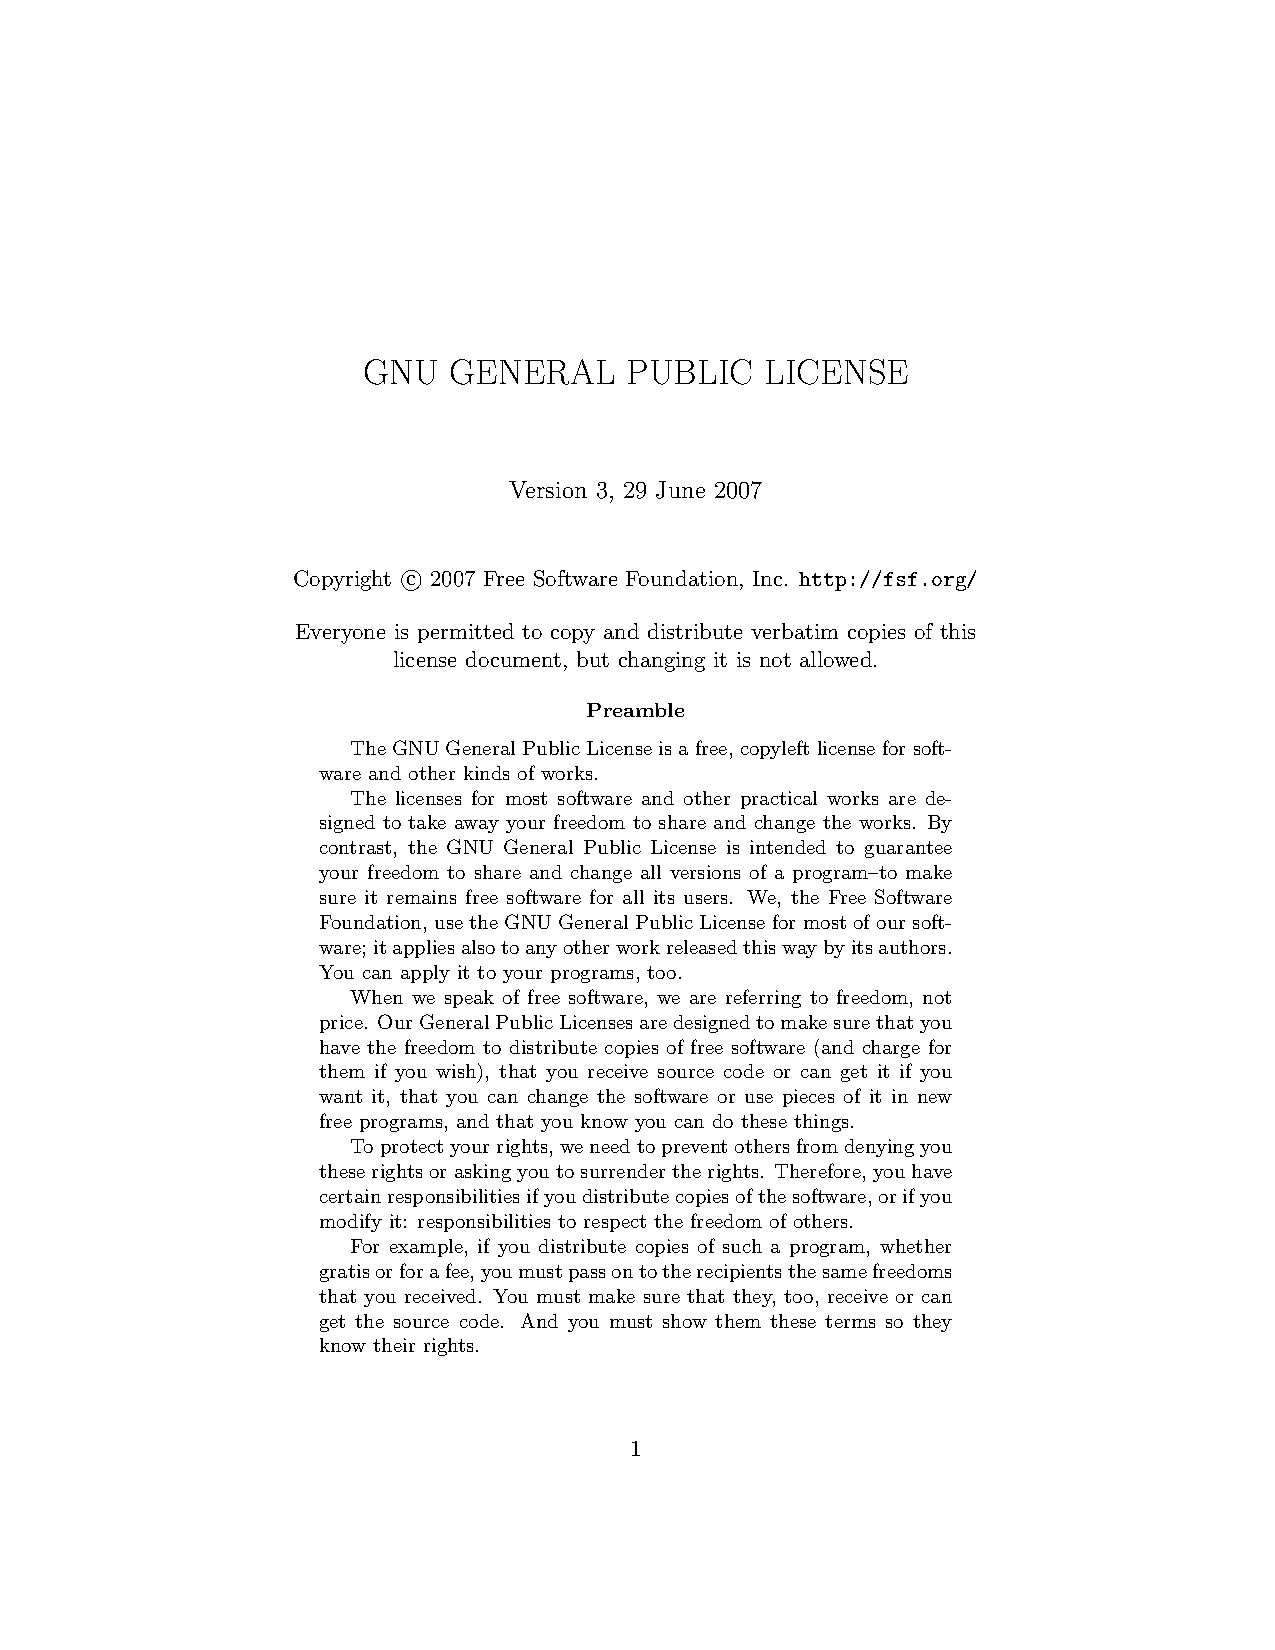
\includepdf[pages={-}]{./LICENCES/gpl.pdf}

\end{document}

